\chapter{混合、振動、電気双極子モーメント、場の演算子}

宣伝された主題から少し外れて、ニュートリノに関する問いから始めよう。ニュートリノが質量を持ち、ニュートリノの種類が混合するという証拠がある。もし質量がすべて同じでないなら、エネルギー保存則に反することなく、どのようにしてある種類が別の種類に変わりうるのだろうか。

この問いは、量子力学の全体に現れるパターンを指し示している。すなわち、系が準備されたり検出されたりする状態は、そのハミルトニアンを対角化する状態である必要はない。確定したエネルギーを持つ状態は位相を得るだけである。いくつかのエネルギーの重ね合わせである準備された状態は、その成分が異なる位相を得るために変化する。この区別が、二重井戸からニュートリノ振動やスピン歳差運動へと我々を導くであろう。電子電気双極子モーメントについての間奏の後、我々は第二量子化に戻り、演算子のレベルで同じ位置--運動量のフーリエ構造を見るであろう。

\section{混合こそが本質的な問題}

ニュートリノがすべて同じ質量を持つ必要はない。エネルギー固有状態は互いに混合しない。それぞれが独立に発展する。ニュートリノの\emph{種類}、すなわちフレーバーと呼ばれるものは、それがどのように生成され検出されるかに関連しており、フレーバー状態は質量エネルギー固有状態の線形結合でありうる。模式的には、
\begin{equation}
|\text{type}\rangle = \sum_n c_n |E_n\rangle .
\end{equation}
したがって正しい言明は、エネルギー固有状態が互いに変化するということではなく、``電子ニュートリノ''や``ミューニュートリノ''と呼ばれる状態がそれ自体エネルギー固有状態である必要はないということである。

\begin{classroomqa}
\lecturetimestamp{00:00:09}
\audiencequestion{もしニュートリノが異なる質量を持つなら、エネルギーが保存されたままで、どのようにして混合しうるのですか。}
\lecturerresponse{質量エネルギー固有状態は互いに変化しない。電子、ミュー、タウのフレーバー状態は、それらの固有状態の異なる線形結合である。各質量成分はそれ自身の位相で発展し、干渉がエネルギー保存則に反することなくフレーバー確率を変化させる。}
\end{classroomqa}

この構造の例は数多くある。最も目に見える例は、対称な二重井戸中の粒子から始まる。

\section{対称な二重井戸と近似的な局在状態}

二つの極小の間に高い障壁がある対称な二重井戸ポテンシャル中を運動する粒子を考えよう。もし障壁が無限に高いとすれば、左と右の井戸は完全に切り離されるであろう。右の井戸が存在しないかのように左の井戸を解くことができ、右の井戸についても同様である。そのとき近似的な基底状態波動関数は、左に局在した状態\(\psi_L\)と右に局在した状態\(\psi_R\)であり、両者は同じエネルギー\(E\)を持つであろう。

それぞれの孤立した井戸において、基底状態はおなじみの定性的性質を持つ。すなわち、滑らかであり、節を持たず、閉じ込めと整合する最も低い可能なエネルギーにある。高い中央の障壁をれんがの壁と考えよう。それを無限と扱うのは近似にすぎないが、そこから始めるのに有用な一対の局在状態を与えてくれる。

\begin{figure}
\centering
\begin{adjustbox}{max width=\linewidth}
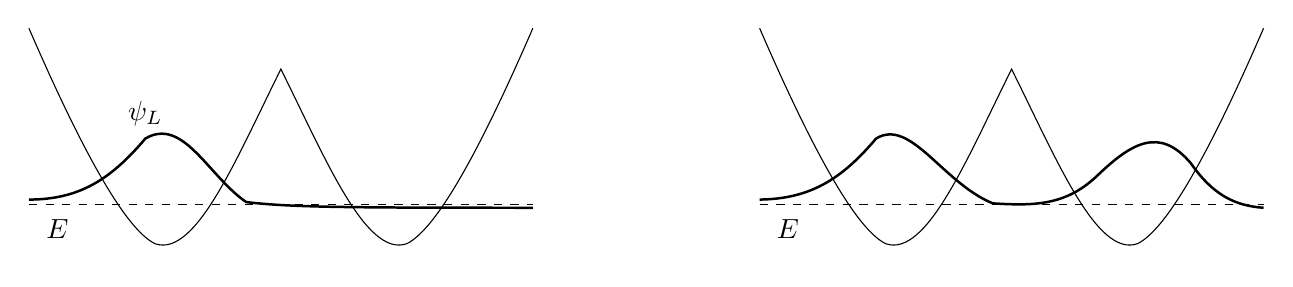
\begin{tikzpicture}[x=0.8cm,y=0.8cm]
\begin{scope}[shift={(-5.8,0)}]
\draw (-4,2.7) .. controls (-3.35,1.2) and (-2.55,-0.45) .. (-2.0,-0.72)
      .. controls (-1.35,-0.95) and (-0.7,0.65) .. (0,2.05)
      .. controls (0.7,0.65) and (1.35,-0.95) .. (2.0,-0.72)
      .. controls (2.55,-0.45) and (3.35,1.2) .. (4,2.7);
\draw[dashed] (-4,-0.10) -- (4,-0.10);
\node at (-3.55,-0.48) {$E$};
\draw[line width=0.9pt] (-4,-0.02) .. controls (-3.2,-0.02) and (-2.7,0.30) .. (-2.15,0.95)
      .. controls (-1.55,1.30) and (-1.15,0.35) .. (-0.55,-0.06)
      .. controls (0.15,-0.14) and (0.9,-0.15) .. (4,-0.15);
\node at (-2.15,1.35) {$\psi_L$};
\end{scope}
\begin{scope}[shift={(5.8,0)}]
\draw (-4,2.7) .. controls (-3.35,1.2) and (-2.55,-0.45) .. (-2.0,-0.72)
      .. controls (-1.35,-0.95) and (-0.7,0.65) .. (0,2.05)
      .. controls (0.7,0.65) and (1.35,-0.95) .. (2.0,-0.72)
      .. controls (2.55,-0.45) and (3.35,1.2) .. (4,2.7);
\draw[dashed] (-4,-0.10) -- (4,-0.10);
\node at (-3.55,-0.48) {$E$};
\draw[line width=0.9pt] (-4,-0.02) .. controls (-3.2,-0.01) and (-2.7,0.30) .. (-2.15,0.95)
      .. controls (-1.6,1.28) and (-1.1,0.25) .. (-0.30,-0.08)
      .. controls (0.35,-0.12) and (0.85,-0.12) .. (1.35,0.35)
      .. controls (1.9,0.88) and (2.35,1.15) .. (2.85,0.55)
      .. controls (3.2,0.05) and (3.55,-0.12) .. (4,-0.15);
\end{scope}
\end{tikzpicture}
\end{adjustbox}
\caption{冒頭の板書スケッチをきれいに描き直したもの。左側は、障壁が実効的に無限であると仮定して得られた片側の試行状態\(\psi_L\)である。右側では、同じ波動関数が障壁を通して対称に延長されており、最終的に真の偶基底状態を生み出す小さくしかし非零の漏れを示している。}
\end{figure}

しかし量子力学的には、障壁は真に無限ではない。障壁領域の波動関数は厳密にゼロではなく、ただ非常に小さいだけである。この微小な漏れがすべてである。これが左右の近似を真の混合問題へと変えるのである。

\section{パリティ固有状態と指数的な準位分裂}

ここで局在の描像は一つの定理によって中断される。すなわち、ポテンシャルが対称ならば、厳密なエネルギー固有関数は反射の下で対称または反対称のいずれかになるように選ぶことができる。

\begin{theorem}
もし一次元で\(V(x)=V(-x)\)ならば、ハミルトニアンの固有関数は次のいずれかを満たすように選ぶことができる。
\[
\psi(x)=\psi(-x)
\qquad \text{or} \qquad
\psi(x)=-\psi(-x).
\]
\end{theorem}

ここで修正が入る。片側の状態\(\psi_L\)と\(\psi_R\)は対称でも反対称でもないので、完全なハミルトニアンの厳密な固有状態にはなりえない。それらは障壁が高いときにのみ良い近似状態である。真の固有状態は対称および反対称の組み合わせであり、
\begin{align}
\psi_+ &= \frac{\psi_L+\psi_R}{\sqrt{2}},\\
\psi_- &= \frac{\psi_L-\psi_R}{\sqrt{2}}.
\end{align}
板書に残る記法を用いて、それらのエネルギーを次のように表す。
\begin{align}
H\psi_+ &= (E_1-\epsilon)\psi_+,\\
H\psi_- &= (E_1+\epsilon)\psi_-.
\end{align}
したがって全分裂は
\begin{equation}
\Delta E = (E_1+\epsilon)-(E_1-\epsilon)=2\epsilon .
\end{equation}

\begin{figure}[htbp]
\centering
\includegraphics[width=0.92\linewidth]{lecture_08_frame_02.png}
\caption{二重井戸ポテンシャルにおける対称的に延長された波動関数。その振幅は障壁の下で小さいがゼロではなく、これが準位分裂の起源である。}
\lectureframe{00:06:19}
\end{figure}

\begin{figure}
\centering
\begin{tikzpicture}[x=1cm,y=1cm]
\draw[->] (0,0) -- (0,3);
\node[left] at (0,2.8) {energy};
\draw (-0.35,1.60) -- (0.35,1.60);
\node[left] at (-0.45,1.60) {$\psi_L,\psi_R$};
\node at (1.7,1.60) {$\Longrightarrow$};
\draw (3.0,1.32) -- (3.75,1.32);
\draw (3.0,1.88) -- (3.75,1.88);
\draw[dashed] (2.8,1.60) -- (3.95,1.60);
\node[right] at (3.9,1.32) {$\psi_+,\ E_1-\epsilon$};
\node[right] at (3.9,1.88) {$\psi_-,\ E_1+\epsilon$};
\node[below] at (3.37,1.60) {$E_1$};
\end{tikzpicture}
\caption{トンネル分裂の板書の論理。近似された左状態と右状態はほとんど縮退しているが、厳密な対称固有状態と反対称固有状態は小さな量\(2\epsilon\)だけ分裂している。}
\end{figure}

準位の順序が物理的な要点を担っている。対称状態は障壁領域を通してより滑らかであるため、エネルギーがわずかに低い。波動関数が漏れ出して対称的に続くことを許すと、エネルギーがほんのわずか下がる。反対称状態はわずかに高い。一次元における第一励起状態は節を一つ持ち、この対称な問題ではその節が中点に位置するからである。余分な曲率は運動エネルギーを消費する。

この効果は非常に小さく、障壁の幅と高さに対して指数的に小さい。ここで明示的なWKBの公式は必要ない。重要な点は、分裂が実在するがごく小さいということである。また、波動関数の全体的な符号は物理的な情報を担わないことを思い出そう。\(\psi_-\)を\(-\psi_-\)に置き換えても状態は変わらない。

\section{時間発展と左右振動}

次に動的な問いを立てよう。粒子を左側の井戸に置いたら何が起こるか。これが決定的な一歩である。振動は、同じ混合現象の時間依存の側面だからである。

逆関係は
\begin{align}
\psi_L &= \frac{\psi_+ + \psi_-}{\sqrt{2}},\\
\psi_R &= \frac{\psi_+ - \psi_-}{\sqrt{2}}.
\end{align}
である。したがって、初期に左に局在した状態は
\begin{equation}
\psi(0)=\psi_L=\frac{\psi_+ + \psi_-}{\sqrt{2}}.
\end{equation}
である。これはエネルギー固有状態ではない。したがって、非自明に発展しなければならない。

我々は標準的なSchr\"odingerの規約\(e^{-iEt}\)を用いる。共通の位相は観測可能な効果を持たない。一方の井戸から他方の井戸へ確率を移動させることができるのは、二つのエネルギー成分の間の相対位相だけである。

この規約では、
\begin{equation}
\psi(t)=\frac{1}{\sqrt{2}}\left(e^{-i(E_1-\epsilon)t}\psi_+ + e^{-i(E_1+\epsilon)t}\psi_-\right).
\end{equation}
である。これが板書の公式を整理したものである。ここで共通の位相をくくり出す。
\begin{equation}
\psi(t)=\frac{e^{-iE_1 t}}{\sqrt{2}}\left(e^{i\epsilon t}\psi_+ + e^{-i\epsilon t}\psi_-\right).
\end{equation}
一方の位相は単位円を一方向に回り、他方の位相は反対方向に回る。状態が変化するのは、これら二つの位相が歩調を外すからにほかならない。

左右振動を明示的に見るために、\(\psi_\pm\)の定義を代入する。
\begin{align}
\psi(t)
&= \frac{e^{-iE_1 t}}{2}
\left[e^{i\epsilon t}(\psi_L+\psi_R)+e^{-i\epsilon t}(\psi_L-\psi_R)\right] \\
&= \frac{e^{-iE_1 t}}{2}
\left[(e^{i\epsilon t}+e^{-i\epsilon t})\psi_L+(e^{i\epsilon t}-e^{-i\epsilon t})\psi_R\right] \\
&= e^{-iE_1 t}\left[\psi_L\cos(\epsilon t)+i\,\psi_R\sin(\epsilon t)\right].
\end{align}
これがこの章の鍵となる計算による導出である。二状態近似において、\(\psi_L\)と\(\psi_R\)が正規直交であるとき、確率は
\begin{equation}
P_L(t)=\cos^2(\epsilon t),
\qquad
P_R(t)=\sin^2(\epsilon t).
\end{equation}
である。したがって、系は振動する。中間の時刻では、系は真に重ね合わせの状態にある。たとえば、\(\epsilon t=\pi/4\)のとき、両側の確率は等しい。位相は連続的に発展し、局在はそれらとともに連続的に変化する。

黒板での導出は、相対符号が反転する最初の時刻を切り出す。いつ
\begin{equation}
e^{-i\epsilon t}=-\,e^{i\epsilon t},
\end{equation}
となるかを問う。これが黒板上の目に見える節目である。両辺に掛け合わせると
\begin{equation}
e^{2i\epsilon t}=-1.
\end{equation}
となる。最初の発生に対しては、
\begin{equation}
2\epsilon t=\pi,
\qquad\text{so}\qquad
t_{L\to R}=\frac{\pi}{2\epsilon}.
\end{equation}

\begin{figure}[htbp]
\centering
\includegraphics[width=0.94\linewidth]{lecture_08_frame_05.png}
\caption{黒板上の相対位相の計算。二つのエネルギー成分は\(e^{2i\epsilon t}=-1\)のとき反対になり、最初の移動時間\(2\epsilon t=\pi\)を与える。組版された導出では一貫した一つのSchr\"odinger位相の規約を用いる。}
\lectureframe{00:17:52}
\end{figure}
その瞬間、
\begin{equation}
\psi(t_{L\to R}) \propto \frac{\psi_+-\psi_-}{\sqrt{2}}=\psi_R.
\end{equation}
全体の位相は無関係である。重要なのは、初めに左側に置かれた粒子が右側に局在した状態へと発展したことである。さらに等しい時間間隔の後、それは再び振り戻る。混合と振動は相伴うものである。

この方程式は曖昧さがない。小さな\(\epsilon\)は遅い振動と長い移動時間を意味する。どちらの局在状態も確定したエネルギーを持たないが、二つの厳密なエネルギー成分はエネルギーを保存し、あるべきとおりに厳密に発展する。

\section{ニュートリノ、アンモニア、スピンの類推}

二重井戸は、元々のニュートリノの問いに対する雛形を与える。電子とともに生成されたニュートリノは電子ニュートリノと呼ばれる。ミューオンとともに生成されたものはミューニュートリノと呼ばれる。これらのフレーバーラベルは生成と検出のチャネルを記述する。確定した質量を持ち、したがって固定された運動量で確定した自由粒子エネルギーを持つ状態は、別の基底をなす。

最も単純な二状態、最大混合の戯画では、
\begin{equation}
|\nu_e\rangle \sim \frac{|m_1\rangle+|m_2\rangle}{\sqrt{2}},
\qquad
|\nu_\mu\rangle \sim \frac{|m_1\rangle-|m_2\rangle}{\sqrt{2}},
\end{equation}
である。ここで質量固有状態は\(\psi_+\)と\(\psi_-\)の役割を果たし、フレーバー状態は\(\psi_L\)と\(\psi_R\)の役割を果たす。実際のニュートリノ混合はこれらの等しい係数ではなく非自明な混合行列を用いるが、機構はすでにここに見えている。

電子ニュートリノは、電子が関与する過程で生成される。ちょうど粒子を左の井戸に放り込むことができるのと同じである。短い飛行距離では、その2つの質量成分はほとんど同じ位相を蓄積しているため、相互作用は依然としてそれを電子フレーバーと同定する。長い基線長では、それらの位相は分離する。その後の荷電カレント相互作用は、電子ではなくミューオンを生成しうる。すなわち、状態はミューフレーバー成分を獲得したのである。異なる距離やエネルギーで実験を繰り返すと、振動が明らかになる。

エネルギー保存則との矛盾はない。質量エネルギー固有状態は、固有状態が行うべきことを正確に行う。フレーバーの重ね合わせ状態が発展するのである。相対論的極限では、観測可能な相対位相は質量二乗差によって支配され、模式的には
\begin{equation}
\Delta\phi_{ij}\simeq \frac{\Delta m_{ij}^{,2}L}{2E}.
\end{equation}
となる。したがって振動は、すべてのニュートリノ質量が同一でありえないことを示している。少なくとも2つの質量固有状態は質量が異なる。

\begin{classroomqa}
\lecturetimestamp{00:24:06}
\audiencequestion{二重井戸の例における小さな分裂\(\epsilon\)を決めるものは何か。}
\lecturerresponse{それは粒子の質量と、障壁の高さおよび幅に依存する。トンネル効果はそれらの詳細に指数的に敏感であるため、障壁のわずかな変化が\(\epsilon\)に大きな割合の変化を生じうる。}
\end{classroomqa}

\begin{classroomqa}
\lecturetimestamp{00:24:26}
\audiencequestion{この振動現象は実際に観測されているのか。}
\lecturerresponse{はい。トンネル分裂は通常の量子系で観測されており、フレーバー振動はニュートリノで観測されている。機構は微視的には異なるが、どちらも同じ2状態の位相発展を実現している。}
\end{classroomqa}

\begin{classroomqa}
\lecturetimestamp{00:24:34}
\audiencequestion{ニュートリノ振動はニュートリノ質量とどのように結びついているのか。}
\lecturerresponse{伝播する固有状態は異なる質量をもち、したがって異なる位相を蓄積する。それらの干渉がフレーバー組成を変化させる。現実的な相対論的取り扱いでは、振動を支配するのは質量二乗差であり、1つの粒子の文字通りの時間変化する質量ではない。}
\end{classroomqa}

\begin{classroomqa}
\lecturetimestamp{00:25:02}
\audiencequestion{ニュートリノ質量は単に有力な理論なのか、それとも実験的事実なのか。}
\lecturerresponse{振動は実験的事実であり、それは非零の質量差を必要とする。絶対質量スケールは別個の、より困難な測定であるが、すべてのニュートリノが質量ゼロであるという最小限の描像は実験的に排除されている。}
\end{classroomqa}

\subsection{アンモニア反転：文字通りの障壁}

アンモニア分子\(\mathrm{NH}_3\)は三角錐形である。3つの水素原子が平面を形成し、窒素はその平面の一方の側にある。窒素が反対側にある等価な配置が存在する。2つの局在化した配置は正確な定常状態ではない。窒素は水素平面を通り抜けてトンネルすることができ、対称および反対称のエネルギー固有状態と小さな反転分裂を生じる。これがアンモニアメーザーにおける同じ数学の物理的起源である。

\begin{classroomqa}
\lecturetimestamp{00:25:11}
\audiencequestion{アンモニアでは、障壁とは窒素が水素平面を通り抜ける配置のことか。}
\lecturerresponse{はい。分子エネルギーはどちらの錐形配置でも最小化されるが、平面配置はより高い。その配置を通り抜けるトンネルが両側を結合する。}
\end{classroomqa}

\begin{classroomqa}
\lecturetimestamp{00:27:10}
\audiencequestion{電子ニュートリノとミューニュートリノの間の対応する物理的障壁は何か。}
\lecturerresponse{文字通りの空間的障壁は存在しない。類推は代数的である。ニュートリノハミルトニアンにおける非対角結合がフレーバー基底を混合する。アンモニアではその結合はトンネル効果から生じるが、ニュートリノではそれは質量と混合の構造の一部である。}
\end{classroomqa}

\subsection{スピン歳差運動：トンネル効果のない混合}

同じ代数はスピンですでに登場している。二つの状態\(|\uparrow_z\rangle\)と\(|\downarrow_z\rangle\)を取る。磁場がなければこれらは縮退している。ここで\(x\)方向に磁場をかける。エネルギー固有状態はもはや\(z\)固有状態ではなく、\(x\)偏極状態である。板書の一時的な左--右という名を用いれば、
\begin{align}
|L_x\rangle &= \frac{|\uparrow_z\rangle+|\downarrow_z\rangle}{\sqrt{2}},\\
|R_x\rangle &= \frac{|\uparrow_z\rangle-|\downarrow_z\rangle}{\sqrt{2}}.
\end{align}
これらは\(\psi_+\)と\(\psi_-\)の直接の類似物である。磁場に平行および反平行に整列した磁気モーメントはわずかに異なるエネルギーをもつ。それらのエネルギーが\(E\mp\epsilon\)であれば、初期に上向きのスピンは次のように発展する：
\begin{equation}
|\uparrow_z,t\rangle
= e^{-iEt}\left[\cos(\epsilon t)\,|\uparrow_z\rangle
+ i\sin(\epsilon t)\,|\downarrow_z\rangle\right].
\end{equation}
これは二重井戸の場合と同じ式であり、ただ今度は連続的発展が\(x\)軸のまわりのスピン歳差運動である。\(+z\)から出発すると、スピンは横方向を通り、歳差運動の半周期後に\(-z\)に達し、さらに半周期後に戻る。\(S_z\)の測定は依然として上か下しか与えない。連続的に変化するスピン状態がそれらの確率を決める。この機構はトンネルを必要としない。必要なのは、ハミルトニアンが準備の基底とは異なる基底で対角的であることだけである。

\begin{classroomqa}
\lecturetimestamp{00:32:25}
\audiencequestion{この描像でタウニュートリノはどうなるのか。}
\lecturerresponse{それも混合する。現実の問題には三つのフレーバー状態と三つの質量状態があり、二状態の回転の代わりに三行三列の混合行列が現れる。位相干渉の原理は変わらない。}
\end{classroomqa}

\begin{classroomqa}
\lecturetimestamp{00:32:57}
\audiencequestion{横磁場をかけた直後、スピンは依然として上向きか、また我々の方向を向くことも反対を向くこともできるのか。}
\lecturerresponse{非常に短い時間では、依然としてほぼ確実に上向きであり、わずかな下向き確率をもつ。状態は磁場軸のまわりを連続的に歳差運動し、横方向\(\pm y\)を通るが、最初に垂直であったなら\(x\)方向の磁場に垂直なままである。どの選んだ軸に沿った測定でも、依然としてその軸の離散固有値の一つを与える。}
\end{classroomqa}

\begin{classroomqa}
\lecturetimestamp{00:34:30}
\audiencequestion{スピンが決して磁場に沿って向かないように、磁場は弱く選ばれているのか。}
\lecturerresponse{いいえ。幾何学は磁場の弱さからではなく、磁場軸のまわりの歳差運動から従う。弱い磁場はエネルギー分裂と歳差運動の振動数を小さくするだけで、ニュートリノの例に類似した遅い振動を与える。}
\end{classroomqa}

ニュートリノ混合の強さと小さなニュートリノ質量は、当初定式化された最小標準模型ではその深い起源が説明されないパラメータである。したがってニュートリノ質量はその最小模型を超えることを示しているが、観測されるスケールは非常に小さく、遠いエネルギー・スケールの物理を反映している可能性がある。

\begin{classroomqa}
\lecturetimestamp{00:36:27}
\audiencequestion{振動がニュートリノに質量があることを知る理由なのか。}
\lecturerresponse{伝播する成分が異なる質量をもつことの決定的な直接的証拠である。関係するすべての成分が厳密に質量ゼロで縮退していれば、質量に依存する相対位相を蓄積せず、この種の真空中のフレーバー振動は起こらない。}
\end{classroomqa}

\begin{classroomqa}
\lecturetimestamp{00:37:57}
\audiencequestion{半周期では、ニュートリノは半分電子フレーバーのように、半分ミューフレーバーのように振る舞うべきか。}
\lecturerresponse{理想的な対称二状態模型では、等しい確率は確率の全周期の四分の一で起こり、完全な変換は最初の極大で起こる。現実の三フレーバー振動では混合角が等しくなく、複数の振動数、スピン・ヘリシティの制約、物質効果があるため、完全に対称な変換は一般的ではない。}
\end{classroomqa}

\begin{classroomqa}
\lecturetimestamp{00:38:36}
\audiencequestion{質量成分が異なるなら、運動量を保存するために太陽ニュートリノの速度は変化しなければならないのか。}
\lecturerresponse{フレーバー状態は固定された質量をもつ成分のコヒーレントな重ね合わせであり、その質量は時間的に振動する古典的量ではない。共通の運動量による記述では成分はわずかに異なるエネルギーと群速度をもち、共通のエネルギーによる記述ではわずかに異なる運動量をもつ。どちらの規約も、一貫して扱えば同じ観測可能な振動位相を与える。}
\end{classroomqa}

この位相発展が古い太陽ニュートリノ欠損を解決した。初期の検出器は主に電子ニュートリノに感度があったため、電子フレーバーとして太陽を出たニュートリノは一部がミューまたはタウフレーバーとして到着し、そのチャネルから逃れることができた。詳細な太陽の計算には三フレーバー混合と物質効果が含まれるが、概念的な教訓はすでに二重井戸に現れている。準備と伝播は異なる基底を用いるのである。

\section{間奏：電気双極子モーメント、対称性、そして``電子球''の主張}

すでに素粒子現象論について話しているので、ここで形式的な数学から少し離れよう。ある一般向け記事は、電子の電気双極子モーメントの新しい上限を、電子が球であることが示されたと述べて紹介した。このスローガンは三つの異なる問いを混同している。電気双極子モーメントが何を測るのか、量子状態にとって回転対称性が何を意味するのか、そして実験が実際に何を制限したのか、である。

\subsection{何が測定されたのか？}

測定された、というよりむしろ上限がつけられたのは、電子の電気双極子モーメントである。分離した電荷\(\pm q\)に対して、双極子モーメントは
\begin{equation}
\mathbf d = q\,\boldsymbol{\ell},
\end{equation}
であり、\(\boldsymbol{\ell}\)は分離ベクトルである。双極子モーメントが非零であるとは、電荷分布がある中心に対して変位していることを意味する。

しかし電子についての関連する問いは、単に電荷が何か任意の方向に中心からずれているかどうかではない。電子はスピンをもち、したがって軸をもつ。また磁気モーメントをもつ。物理的に意味のある問いは、電荷の変位とその軸との間に相関があるかどうかである：
\begin{equation}
\mathbf d_e \parallel \boldsymbol{\mu}_e
\qquad \text{or equivalently} \qquad
\mathbf d_e \parallel \mathbf S .
\end{equation}
この相関こそが電子の電気双極子モーメントと呼ばれるものである。概念的には、スピン偏極した電子を電場中に置くと二つのスピン方位が分裂するかどうかを問う：
\begin{equation}
H_{\mathrm{EDM}}=-\mathbf d_e\cdot \mathbf E,
\qquad
\mathbf d_e=d_e\frac{\mathbf S}{|\mathbf S|}.
\end{equation}
実際の卓上実験は、コンデンサー板の間にただ電子が置かれているだけの場合よりはるかに微妙であるが、これがその実験が利用している対称性とエネルギーシフトの考え方である。

\subsection{なぜEDMがないことは球を意味しないのか}

第一の修正は初等的である。物体は双極子モーメントをもたなくても、球でないことはありうる。中心をもつ楕円体は一方の側にも他方の側にも同じだけ電荷をもち、したがって双極子をもたないが、四重極モーメントをもつことはありうる。さらに複雑な分布は、双極子も四重極ももたずにより高次の多重極をもつかもしれない。一つの多重極係数を測ることは、形全体を決定しない。

量子力学は``形''という語をより微妙なものにする。ほぼ固定された結合長をもつ二原子の、ダンベル状の分子を想像しよう。動径振動を無視し、回転だけを残す。その回転状態は角運動量でラベルされる。分子がボソン的なら、最低回転状態は\(J=0\)をもつ。角運動量が回転を生成するので、
\begin{equation}
\begin{gathered}
J=0 \quad\Longrightarrow\\
\text{rotationally invariant ground state.}
\end{gathered}
\end{equation}
量子状態は回転不変である。にもかかわらず、あらゆる確定した配向の描像はダンベルのように見える。これをすべての配向のコヒーレントな重ね合わせとして記述してもよい。その状態を``球対称''と呼ぶことは、ある測定には有用で、別の測定には誤解を招く。

素早いスナップショットを撮ろう。スナップショットは配向の測定であり、十分に鋭い配向測定は系を角度について局在した状態に残す。そのような状態は同時に確定した角運動量をもつことはできない。これは位置--運動量不確定性原理の回転版である：角度を局在化することは必然的に角運動量の広がりをもたらし、したがって回転励起をもたらす。

剛体回転子に対して、
\begin{equation}
E_J=\frac{J(J+1)}{2I},
\end{equation}
であるから、分解エネルギーは慣性モーメント\(I\)で制御される。体育館のダンベルは巨大な\(I\)をもち、回転準位は驚くほど近接している。通常の光は容易にそれを乱し、配向を明らかにするのに十分である。分子はより広い準位間隔をもつ。コンパクトなハドロンはさらにずっと広い間隔をもつ。探針が最初の分解可能な回転構造を励起するのに十分なエネルギーをもたなければ、繰り返しの測定は回転平均された基底状態だけを見る。

中間子は、クォーク--反クォークの二体系として大まかに描くことができる。その最初の軌道励起は数億電子ボルト以上を要し、光学光子をはるかに超えている。したがって低エネルギーの探針は、その下にある配向のスナップショットを撮ることができない。``球か否か''は、どの状態が準備されるかについての問いであり、また一部は装置の分解能についての問いである。

電子はこの問題を鋭くする。それはスピン\(\tfrac12\)の粒子であり、回転スカラーではない。スピン偏極した状態は軸と磁気モーメントを担う。その軸の周りを電荷が循環するというおなじみの描像は、単なるヒューリスティックである---点状のディラック粒子は文字通り小さな回転する球ではない---が、磁気モーメントがスピンとともに反転することを正しく思い出させる。EDMの問いは、電気的な電荷の変位が同じ軸と相関しているかどうかを問う。答えがゼロであることは、電子を古典的な球に変えるものではない。

\begin{classroomqa}
\lecturetimestamp{00:57:30}
\audiencequestion{電子の電荷の一部を変位させることは電荷の量子化に反するのか。}
\lecturerresponse{否。電荷の量子化は全電荷を固定する。双極子モーメントはその電荷分布の第一空間モーメント、あるいは等価に、点粒子が電場に結合する許された結合に関わるものであり、全電荷の分数変化を要求するものではない。}
\end{classroomqa}

\begin{classroomqa}
\lecturetimestamp{00:58:00}
\audiencequestion{電気双極子モーメントは量子場の理論によって禁じられるのか。}
\lecturerresponse{量子場の理論そのものによって禁じられるのではない。特定の離散対称性が厳密であるときに禁じられる。それらの対称性が破れれば、EDM演算子は許されるが、その係数は極めて小さくなりうる。}
\end{classroomqa}

\subsection{パリティと時間反転}

EDMの議論の実質的な内容は対称性である。パリティの下で、電気双極子モーメントは通常の極性ベクトルとして振る舞い、磁気モーメントは軸性ベクトルとして振る舞う：
\begin{align}
P:\qquad &\mathbf d_e \to -\mathbf d_e,
&\boldsymbol{\mu}_e \to \boldsymbol{\mu}_e .
\end{align}
時間反転の下では、磁気モーメントを定義する循環電流は反転するが、静的な電気変位は反転しない：
\begin{align}
T:\qquad &\mathbf d_e \to \mathbf d_e,
&\boldsymbol{\mu}_e \to -\boldsymbol{\mu}_e .
\end{align}
したがって、電子のスピン軸に沿った非零のEDMは、厳密なパリティ対称性によっても、厳密な時間反転対称性によっても禁じられる：
\begin{equation}
(P\ \text{exact}) \Rightarrow \mathbf d_e=0,
\qquad
(T\ \text{exact}) \Rightarrow \mathbf d_e=0.
\end{equation}

この幾何学は明示する価値がある。磁気モーメントはループ状の電流によって生じる。鏡映は通常の極性ベクトルを反転させるが、そのループに垂直な軸性ベクトルは変えない。軸に沿った電荷の変位は反転する。したがって、\(\mathbf d_e\)が\(\boldsymbol\mu_e\)に平行な電子は、磁気的配向は同じだが電気モーメントと磁気モーメントの関係が逆である電子へと鏡映されるであろう。パリティが厳密であり、電子種がただ一つしかなければ、二つの記述は同じ粒子を表さなければならない；\(d_e=0\)のみが整合する。

時間反転は別の仕方で同じ結論を与える。フィルムを逆回しにすると電流が反転し、したがって\(\boldsymbol\mu_e\)が反転するが、静的な電荷変位は動かない。モーメントが平行な状態は反平行な状態になる。厳密な時間反転対称性は再び\(d_e=0\)を要求するであろう。

\begin{figure}[htbp]
\centering
\begin{tikzpicture}[>=Stealth,scale=0.95]
  \node[font=\bfseries] at (1.0,2.25) {original};
  \draw[->,very thick,blue!70!black] (0.65,0) -- (0.65,1.65);
  \draw[->,very thick,red!75!black] (1.35,0) -- (1.35,1.65);
  \node[blue!70!black,below] at (0.65,0) {$\boldsymbol\mu$};
  \node[red!75!black,below] at (1.35,0) {$\mathbf d$};

  \node[font=\bfseries] at (4.5,2.25) {parity};
  \draw[->,very thick,blue!70!black] (4.15,0) -- (4.15,1.65);
  \draw[->,very thick,red!75!black] (4.85,1.65) -- (4.85,0);
  \node[blue!70!black,below] at (4.15,0) {$\boldsymbol\mu$};
  \node[red!75!black,below] at (4.85,0) {$-\mathbf d$};

  \node[font=\bfseries] at (8.0,2.25) {time reversal};
  \draw[->,very thick,blue!70!black] (7.65,1.65) -- (7.65,0);
  \draw[->,very thick,red!75!black] (8.35,0) -- (8.35,1.65);
  \node[blue!70!black,below] at (7.65,0) {$-\boldsymbol\mu$};
  \node[red!75!black,below] at (8.35,0) {$\mathbf d$};
\end{tikzpicture}
\caption{黒板の議論から再構成された対称性の検証。パリティは電気双極子を反転させるが軸性磁気モーメントは反転させない；時間反転は磁気モーメントを反転させるが静的な電気変位は反転させない。いずれかの厳密な対称性がスピンに平行な永続的EDMを禁じる。}
\end{figure}

\begin{figure}[htbp]
\centering
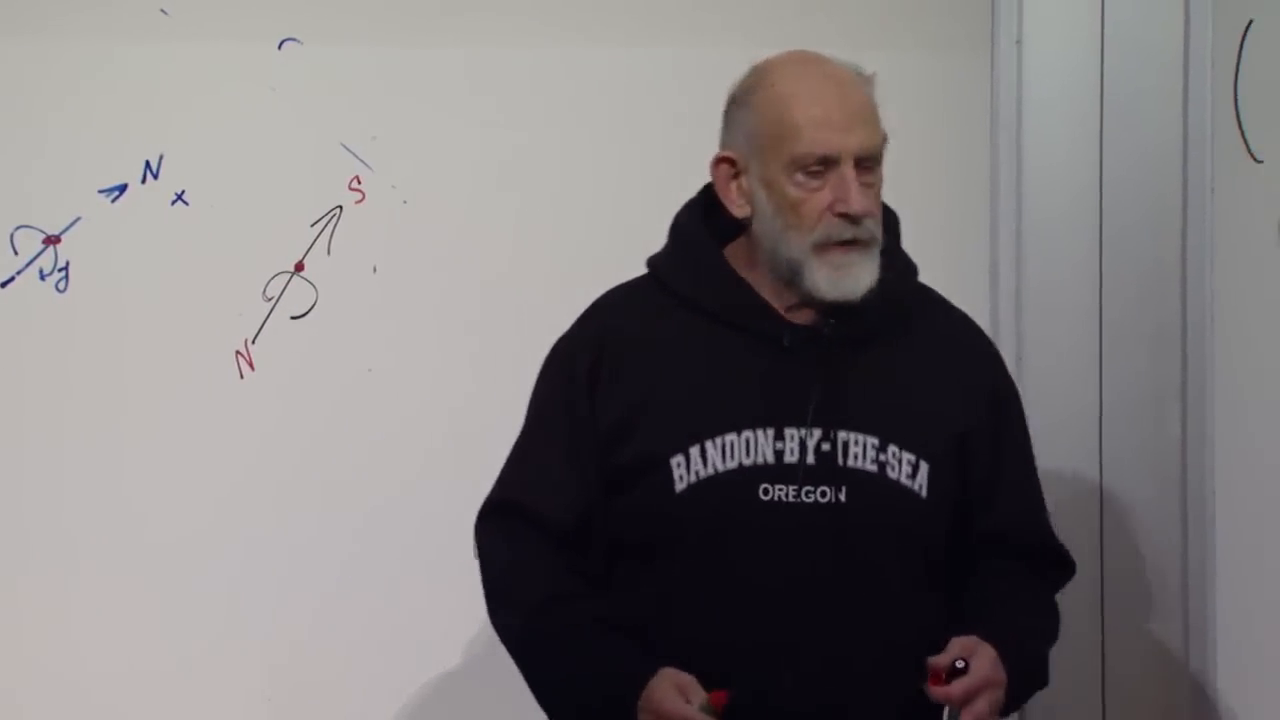
\includegraphics[width=0.94\linewidth]{lecture_08_frame_06.png}
\caption{時間反転の議論の際の、磁気軸と電荷変位の対になったスケッチ。上の簡潔なTikZ図は、部分的に消された生の黒板から変換内容を切り出したものである。}
\lectureframe{01:06:10}
\end{figure}

\begin{classroomqa}
\lecturetimestamp{01:06:38}
\audiencequestion{時間反転の下で、電流と電荷の両方が反転するのか。}
\lecturerresponse{電流は速度が反転するために反転する；電荷そのものは反転しない。電荷の符号を反転させるのは電荷共役\(C\)であり、時間反転\(T\)ではない。}
\end{classroomqa}

\begin{classroomqa}
\lecturetimestamp{01:07:01}
\audiencequestion{時間反転の反ユニタリ性は、非相対論的量子力学が時間反転不変でないことを意味するのか。}
\lecturerresponse{否。反ユニタリ性は、時間反転が量子力学において整合的に表現されるまさにその方法である：それは振幅を複素共役にし、運動量とスピンを反転させる。特定のハミルトニアンが不変であるかどうかは別の問題である。}
\end{classroomqa}

\begin{classroomqa}
\lecturetimestamp{01:07:19}
\audiencequestion{EDMの議論には、電子が点状ではなく有限の体積を持つことが必要か。}
\lecturerresponse{否。点粒子の有効ハミルトニアンは\(-d_e\,\widehat{\mathbf S}\!\cdot\!\mathbf E\)を含みうる。実験は、反対向きのスピン配向が異なる電場エネルギーを得るかどうかを問うのであり、文字通りの広がった電荷雲を分解する必要はない。}
\end{classroomqa}

パリティは弱い相互作用の対称性ではない；それはそれらのカイラル結合において可能な限り強く破れている。時間反転もまた厳密ではないが、標準模型における既知の破れが電子EDMに寄与するのは極めて小さなレベルにおいてのみである。非零の標準模型の寄与を計算することはできるが、それはここで議論した感度のはるかに下にある。したがって、ヌル結果は標準模型と整合しつつ、はるかに大きな時間反転の破れを生みうる拡張---例えば超対称性やその他の新しい相互作用---に切り込むものである。

基本的な実験的発想は単純である。磁場はスピンの向きを分裂させることによって磁気双極子を明らかにする。電場は、スピンに相関した追加のエネルギーシフトによってEDMを明らかにするであろう。実際の精密実験は、素朴な装置の中の孤立した電子ではなく、原子や分子、長いコヒーレント歳差時間、印加磁場の反転、そして系統誤差の注意深い制御を用いる。

\begin{classroomqa}
\lecturetimestamp{01:11:02}
\audiencequestion{EDM探索は高エネルギー衝突実験であったのか、それとも物質的な対象を用いた実験であったのか。}
\lecturerresponse{それは、制御された原子または分子環境に束縛された電子を、電場および磁場とともに用いる精密な卓上物理学であった。そのエネルギーは低いが、微小な対称性破れのシフトに対する感度は、高エネルギーの新物理学を間接的に探るものである。}
\end{classroomqa}

\begin{classroomqa}
\lecturetimestamp{01:12:21}
\audiencequestion{このヌル結果は、標準模型のどのような修正がなお実行可能であり続けるかを制約するのか。}
\lecturerresponse{原理的にはそうである。すべての模型は係数を予言し、したがって何らかのパラメータ領域を占める。詳細な数値的排除には専門家による計算が必要であるが、一般的な論理は堅固である---標準模型との一致がより高い精度で得られるほど、大きなEDMを予言する代替案の余地は小さくなる。}
\end{classroomqa}

\begin{classroomqa}
\lecturetimestamp{01:13:09}
\audiencequestion{量子情報の保存には時間反転対称性が必要か。}
\lecturerresponse{いいえ。ハミルトニアンが\(T\)の下で不変でなくても、ユニタリな時間発展は情報を保存する。固定された磁場中の粒子はよく知られた例である。その磁場は、磁場も同時に反転しない限り、時間反転した映画の中で一つの向きを選び出すが、それでも量子発展はユニタリのままである。局所ローレンツ不変量子場理論の通常の仮定の下では、\(CPT\)の結合変換は対称性であるが、それがユニタリ性を保証しているのではない。}
\end{classroomqa}

ここでこの中断を終えることができる。ヌル測定は、述べられた感度において電子に検出されたEDMが存在しないことを述べている。それは電子が球であるとは述べておらず、標準模型を覆すものでもない。それは、その模型からのいくつかの提案された逸脱を持続させることをより難しくする。

\section{第二量子化へ戻る：フーリエ変換、運動量モード、局所性}

我々は第二量子化を行っていた。通常の一粒子波動関数についてのよく知られた事実から穏やかに再開し、それを演算子へと持ち上げよう。フーリエ変換との関係は厳密かつ単純である。

\subsection{位置空間から運動量空間へ}

小文字の\(\psi\)であり、大文字の\(\Psi\)ではないものが、単一粒子の波動関数である。位置空間では、
\begin{equation}
P(x)=|\psi(x)|^2
\end{equation}
は粒子が位置\(x\)に見出される確率密度である。運動量空間の波動関数はそのフーリエ変換であり、
\begin{equation}
\tilde{\psi}(p)=\int dx\,\psi(x)\,\frac{e^{-ipx}}{\sqrt{2\pi}},
\end{equation}
であり、逆関係は
\begin{equation}
\psi(x)=\int dp\,\tilde{\psi}(p)\,\frac{e^{ipx}}{\sqrt{2\pi}}.
\end{equation}
である。このとき
\begin{equation}
P(p)=|\tilde{\psi}(p)|^2
\end{equation}
は運動量\(p\)に対する確率密度である。

我々は\(\hbar=1\)を用いる。二つの変換は逆変換の関係にある。すなわち、どちらか一方の波動関数を知れば他方が定まるが、それらの絶対値の二乗は異なる測定の問いに答える。

自由粒子に対しては、
\begin{equation}
H=\frac{p^2}{2m},
\end{equation}
であるから、運動量固有状態はエネルギー固有状態でもあり、その位置空間の波動関数は平面波である。
\begin{equation}
\psi_p(x)\propto e^{ipx}.
\end{equation}
これが第二量子化版への出発点である。

\begin{figure}[htbp]
\centering
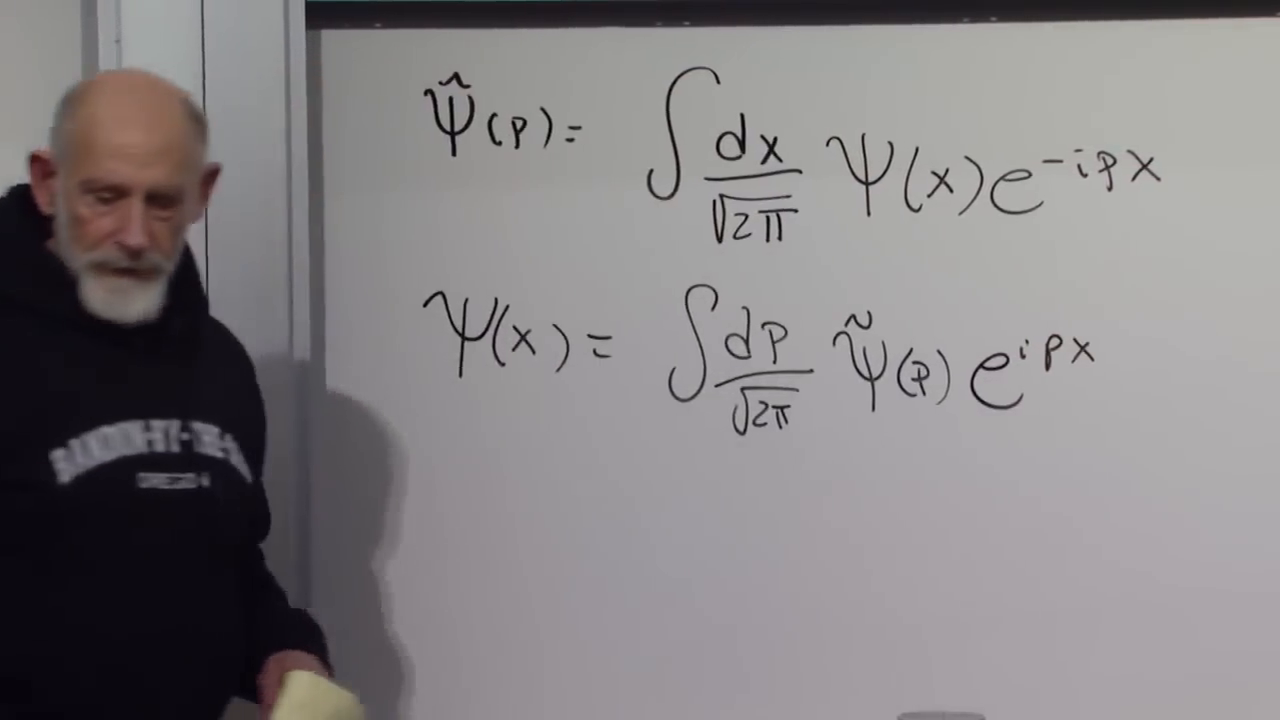
\includegraphics[width=0.94\linewidth]{lecture_08_frame_07.png}
\caption{一粒子波動関数に対する位置--運動量のフーリエ対。小文字の\(\psi\)と、次に導入される大文字の場の演算子との区別は本質的である。}
\lectureframe{01:20:00}
\end{figure}

\subsection{位置空間および運動量空間における場の演算子}

さて場の演算子に戻ろう。黒板ではその消滅部分と生成部分が\(\Psi_-(x)\)および\(\Psi_+(x)\)と書かれている。しばらくその記法を保つと、
\begin{align}
\Psi_-(x) &= \sum_i a_i\,\psi_i(x),\\
\Psi_+(x) &= \sum_i a_i^\dagger\,\psi_i^*(x).
\end{align}
ここで\(\psi_i(x)\)は\(i\)番目のモードの通常の一粒子波動関数であり、\(a_i\)と\(a_i^\dagger\)はそのモードの粒子を消滅および生成する。この時点から、次のように改名するのが便利である。
\[
\Psi(x)\equiv \Psi_-(x),
\qquad
\Psi^\dagger(x)\equiv \Psi_+(x).
\]

自由粒子に対しては、離散的なモードラベル\(i\)は連続的な運動量ラベル\(p\)に置き換えられる。平面波\(e^{ipx}\)を用いると、標準的な再構成された公式が得られる。
\begin{align}
\Psi(x) &= \int \frac{dp}{\sqrt{2\pi}}\,a(p)\,e^{ipx},\\
\Psi^\dagger(x) &= \int \frac{dp}{\sqrt{2\pi}}\,a^\dagger(p)\,e^{-ipx}.
\end{align}
これらは通常のフーリエ変換の場の演算子版である。それらは以前とまったく同様に厳密に逆変換できる。
\begin{align}
a(p) &= \int \frac{dx}{\sqrt{2\pi}}\,\Psi(x)\,e^{-ipx},\\
a^\dagger(p) &= \int \frac{dx}{\sqrt{2\pi}}\,\Psi^\dagger(x)\,e^{ipx}.
\end{align}
\(1/\sqrt{2\pi}\)の因子は、順変換と逆変換が同じ規格化をもつように選ばれた慣習である。

概念的な内容は単純である。\(\Psi^\dagger(x)\) は位置 \(x\) に粒子を生成し、\(a^\dagger(p)\) は運動量 \(p\) を持つ粒子を生成する。位置空間と運動量空間の生成演算子は互いにフーリエ共役であり、通常の量子力学において \(\psi(x)\) と \(\tilde{\psi}(p)\) がフーリエ共役であるのと同じである。

運動量 \(p\) の粒子が存在しなければ、\(a(p)\) はその状態を消滅させる。その運動量の粒子が存在すれば、通常の占有数係数とともに一つを除去する。同様に、\(\Psi(x)\) は \(x\) にある粒子を除去し、これは分布的あるいは波動束に塗り込んだ後に理解される。各粒子種はそれぞれ独自の場の演算子を必要とし、一つの場があらゆる種類の粒子を生成することはできない。

\subsection{ボソンの交換関係と離れた測定の独立性}

次の事実は定義から直接導出できる。ボソンに対して、
\begin{equation}
[a_i,a_j^\dagger]=\delta_{ij},
\qquad
[a_i,a_j]=0,
\qquad
[a_i^\dagger,a_j^\dagger]=0.
\end{equation}
連続版は
\begin{equation}
[a(p),a^\dagger(p')]=\delta(p-p').
\end{equation}
である。ここで離散展開から等時場の交換関係を計算する：
\begin{align}
[\Psi(x),\Psi^\dagger(y)]
&= \sum_{i,j}\psi_i(x)\psi_j^*(y)\,[a_i,a_j^\dagger] \\
&= \sum_i \psi_i(x)\psi_i^*(y) \\
&= \delta(x-y),
\end{align}
ここで最後のステップは一粒子基底の完全性を用いている。同様に、
\begin{equation}
[\Psi(x),\Psi(y)]=0,
\qquad
[\Psi^\dagger(x),\Psi^\dagger(y)]=0.
\end{equation}

\begin{figure}[htbp]
\centering
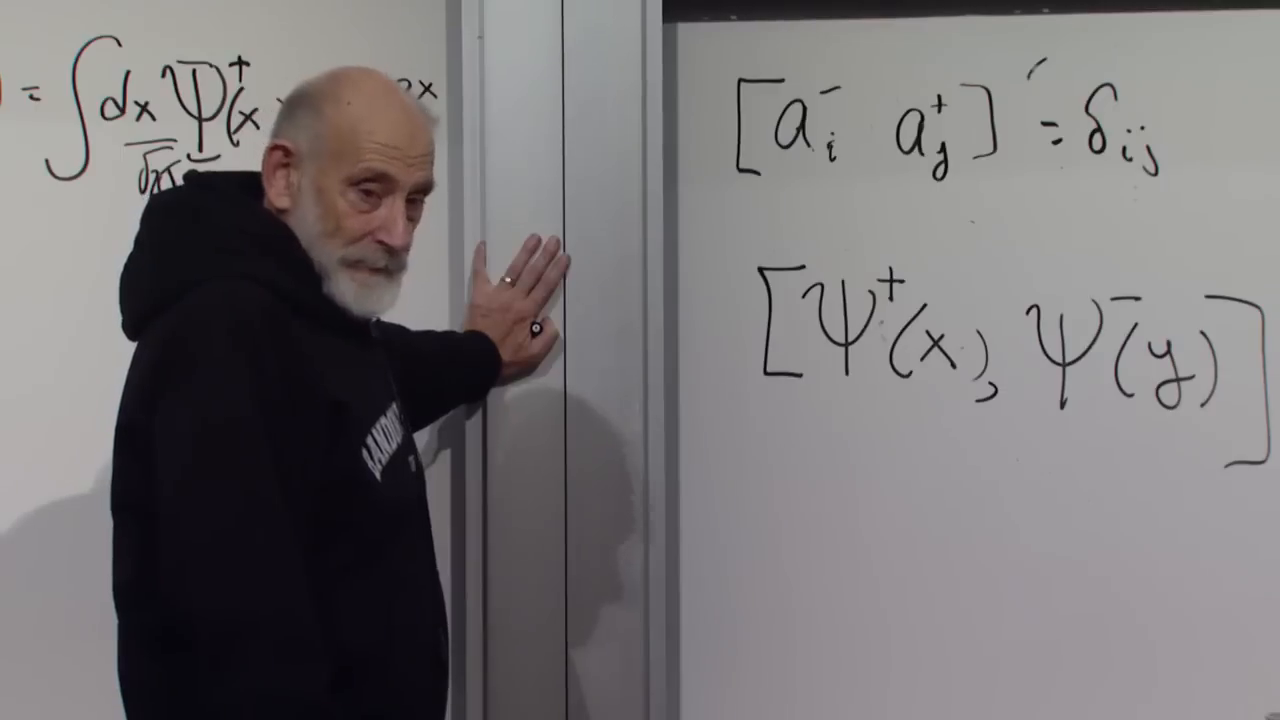
\includegraphics[width=0.94\linewidth]{lecture_08_frame_08.png}
\caption{モードの交換関係とその位置空間における対応物を黒板に示す。完全性により \(\delta_{ij}\) は空間的デルタ分布 \(\delta(x-y)\) になる。}
\lectureframe{01:31:00}
\end{figure}

重要な点は単に \(\Psi\) が非エルミートであることではない。エルミートな直交成分を定義する：
\begin{equation}
Q(x)=\frac{\Psi(x)+\Psi^\dagger(x)}{\sqrt{2}},
\qquad
P(x)=\frac{\Psi(x)-\Psi^\dagger(x)}{i\sqrt{2}}.
\end{equation}
それらの同一点における交換関係はデルタ分布を受け継ぐ。したがって、二つの局所直交成分は位置と運動量が共役であるのと同じ意味で共役である。一方を鋭くしようとすると他方に不確定性が生じる。

\begin{classroomqa}
\lecturetimestamp{01:32:03}
\audiencequestion{\(x=y\) のときデルタ関数は何を意味するのか。交換関係はどこでも大きいのか。}
\lecturerresponse{デルタは分布であり、有限の点値を持つ通常の関数ではない。引数が離れていれば消え、試験関数との積分の後にのみ有限の結果を与える。有限の検出器領域にわたり場を塗り込むと、形式的な同一点の特異性は二つのモードの通常の有限な正準交換関係になる。}
\end{classroomqa}

しかし \(x\neq y\) に対しては、等時交換関係は消える。二つの互いに素な領域に局在する操作は独立に実行できる：ここで場を測定しても、そこでの場に量子的なキックを与えない。これは相対論的微視的因果性の非相対論的な等時先駆である。相対論的理論では、物理的な局所可観測量は空間的隔たりで交換し、そこでは光信号が二つの事象を結ぶことができない。

非可換な可観測量との対比はよく知られている。\([x,p]=i\) であるから、精密な位置測定は運動量を乱し、精密な運動量状態は位置において広がる。異なるスピン成分が交換しないため、一つの成分を鋭く準備すると別の成分が不確定になる。離れた局所可観測量間の非零の交換関係は、同様に、一方の領域での操作が他方を乱すことを意味し、要求される因果的独立性と矛盾する。

\begin{classroomqa}
\lecturetimestamp{01:37:51}
\audiencequestion{EPR とエンタングルメントの実験は、ここでの測定が遠方の測定に影響を与えることを示すのか。}
\lecturerresponse{それらは相関を示すのであり、制御可能な因果的影響を示すのではない。エンタングルした結果は古典的因数分解を破るが、遠方の検出器における局所統計は、ここでの測定の選択や実行によって変えることはできない。空間的に離れた可観測量の交換関係は、そのノーシグナリング独立性の背後にある演算子としての言明である。}
\end{classroomqa}

次回は代数が変わる。フェルミオンの生成消滅演算子は反交換関係を満たす。素朴に考えると、離れた点におけるフェルミオン場は交換しないので、場自体を直接測定可能なボソン的可観測量として解釈することはできない。物理的なフェルミオン的可観測量は偶の組み合わせ---密度、電流、応力テンソル---であり、それらの局所可観測量は要求される空間的隔たりでの交換性を回復する。これが第二量子化のフェルミオン版への入口である。
